\documentclass[14pt]{beamer}
\usetheme{Warsaw}
\beamertemplatenavigationsymbolsempty

\title{BFS on FPGA}
\author{Nina Engelhardt}
\date{\today}

\begin{document}
	\begin{frame}
		\maketitle
	\end{frame}
\setlength{\parskip}{1em}


\begin{frame}
	\frametitle{Breadth First Search}

	\begin{itemize}
		\addtolength{\itemsep}{0.5\baselineskip}
		\item Find minimal spanning tree
		\item Equivalent to shortest path from root to all nodes, with unweighed edges
		\item For correct parallel implementation, synchronization barrier between ``levels'' is important
	\end{itemize}
\end{frame}

\begin{frame}
	\frametitle{Vertex-Centric Algorithms}
	Distributed, synchronous execution in phases separated by global barriers:
	\vspace{-0.5em}
	\begin{enumerate}
		\item Node receives messages from previous phase
		\item Node updates internal status based on data received
		\item Node sends messages with new data to neighbors for next phase
	\end{enumerate}
	\vspace{-0.5em}
	Nodes are \emph{active} if they receive at least one message in a phase.
	Computation terminates when no active nodes remain.
\end{frame}

\begin{frame}
	\frametitle{Vertex-Centric Algorithms}
	Salient features:
	\vspace{-0.8em}
	\begin{itemize}
		\addtolength{\itemsep}{0.5\baselineskip}
		\item Need to store all messages between phases! Potentially as many as there are edges in the graph.
		\item Need to be able to determine activity/detect termination.
	\end{itemize}
\end{frame}

\begin{frame}
	\frametitle{Implementation}
	\begin{itemize}
		\addtolength{\itemsep}{0.5\baselineskip}
		\item Split nodes across multiple processing elements
		\item NoC interconnect to transfer and store messages
		\end{itemize}
\end{frame}

\begin{frame}
	\frametitle{Implementation: NoC}
	\begin{itemize}
		\addtolength{\itemsep}{0.5\baselineskip}
		\item Currently, just $N \times N$ FIFO queues linking all PEs point-to-point (including self-link)
		\item ``Floating barrier'': assuming in-order delivery of messages, PE signals end of phase by sending a barrier marker
		\item Other PEs will not consume messages in queue behind barrier marker until next phase
		\item PE passes to next phase when barrier marker received from all PEs
	\end{itemize}
\end{frame}

\begin{frame}
	\frametitle{Implementation: PE}
	\begin{minipage}{0.68\textwidth}
	Components:

	\begin{itemize}
		\addtolength{\itemsep}{0.5\baselineskip}
		\item Incoming message queues
		\item Apply module
		\item Update broadcast module
	\end{itemize}
	\end{minipage}
	\begin{minipage}{0.3\textwidth}
		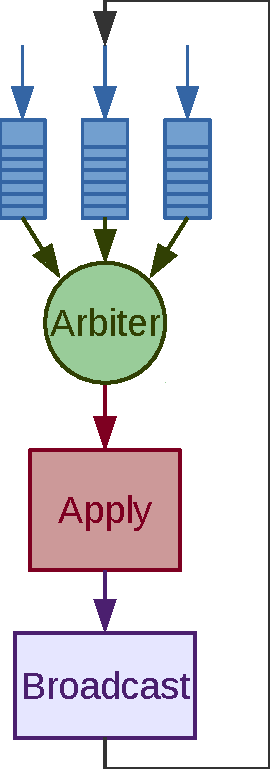
\includegraphics[width=0.8\textwidth]{arch.pdf}
	\end{minipage}
\end{frame}

\begin{frame}
	\frametitle{Implementation: Incoming Messages}
	\begin{itemize}
		\addtolength{\itemsep}{0.5\baselineskip}
		\item $N$ queues buffering messages from each PE
		\item Round-robin consume message from a queue where non-barrier message at front
		\item If all queues show barrier, consume all barrier markers and signal barrier to Apply module
		\item Two barriers in a row = no active nodes in this PE during last phase
	\end{itemize}
\end{frame}

\begin{frame}
	\frametitle{Implementation: Apply}
	\begin{itemize}
		\addtolength{\itemsep}{0.5\baselineskip}
		\item Contains node-associated data storage
		\item Algorithm-specific. In BFS:
		\begin{itemize}
			\item message contains ID of destination node and sender node
			\item check destination node storage. If not yet visited (= 0), store parent information (sender node ID) and output ID of updated node
		\end{itemize}
		\item Barrier messages are passed along to output in order (increase internal counter)
	\end{itemize}
\end{frame}

\begin{frame}
	\frametitle{Implementation: Broadcast}
	\begin{itemize}
		\addtolength{\itemsep}{0.5\baselineskip}
		\item Receives message payload to broadcast and sending node ID (in BFS, both are the same)
		\item Looks up neighbors of sending node in edge storage
		\item Sends message to all neighbors
		\item For barriers, sends barrier marker to all PEs (including self)
	\end{itemize}
\end{frame}

\begin{frame}
	\frametitle{Issues}
	Things to work on near term:
	\vspace{-0.8em}
	\begin{itemize}
		\addtolength{\itemsep}{0.5\baselineskip}
		\item Deadlock if not enough queue space (buffer after apply most space-effective)
		\item Number of PEs vs. PE size - more nodes per PE mean less area overhead, but also less parallelism
		\item Simulation only works up to 64 PEs
	\end{itemize}
\end{frame}

\begin{frame}
	\frametitle{Issues}
	Things to work on long term:
	\vspace{-0.8em}
	\begin{itemize}
		\addtolength{\itemsep}{0.5\baselineskip}
		\item NoC: $N \times N$ FIFO approach not scalable
		\item How to partition nodes across PEs (currently filled in order)
		\item How to deal with nodes with many neighbors (split single node across multiple PE?)
	\end{itemize}
\end{frame}

\begin{frame}
	\frametitle{Some simulation results}
	GRCite graph has 1953 nodes and 8307 edges.\footnote{Due to clustering of high-arity nodes, could not reduce edge storage size going from 2 to 4 PEs.}
	\vspace{-0.8em}
	\begin{center}
	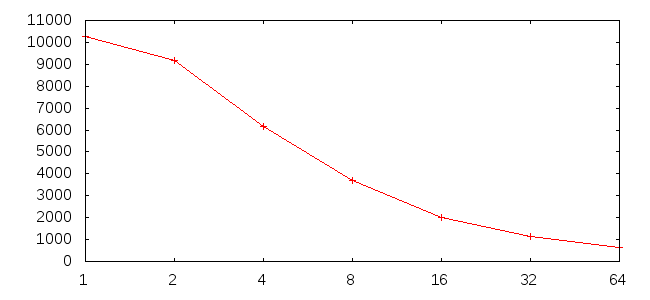
\includegraphics[width=0.95\textwidth]{grcite-numpe.png}
	\end{center}
\end{frame}

\begin{frame}
	\frametitle{Graph density effect on runtime}
	Random connected graph (different one each time) with 32000 nodes and $n$ edges:
	\begin{itemize}
		\addtolength{\itemsep}{0.5\baselineskip}
		\item $n=34000$: 3445 cycles taken.
		\item $n=64000$: 5314 cycles taken.
		\item $n=128000$: 9470 cycles taken.
		\item $n=192000$: 13711 cycles taken.
	\end{itemize}
\end{frame}


\end{document}

%%%%%%%%%%%%%%%%%%%%%%%%%%%%%%%%%%%%%%%%%%%%

\begin{frame}
	\frametitle{}

	\vspace{-0.8em}
	\begin{itemize}
		\addtolength{\itemsep}{0.5\baselineskip}
		\item 
		\item 
		\item 
	\end{itemize}
\end{frame}